\documentclass[runningheads]{llncs}
\usepackage{times}
\usepackage{amsmath}
\usepackage{amssymb}
\usepackage{algorithm}
\usepackage[noend]{algpseudocode}
%\usepackage[ruled,linesnumbered,noend,oldcommands]{algorithm2e}
\usepackage{xspace}
\usepackage{mathtools}
\usepackage{graphicx}
\usepackage{array}
\usepackage{xcolor}
\usepackage{theorem}
\usepackage[T1]{fontenc}
% \usepackage[T1,hyphens]{url}
\usepackage{hyperref}
%\PassOptionsToPackage{hypnens}{url}

\algrenewcommand\algorithmicprocedure{}
\algrenewcommand\algorithmicthen{}
\algrenewcommand\algorithmicdo{}

\newcommand{\fs}[1]{\fontsize{#1}{#1}\selectfont}
\newcommand{\fss}[2]{\fontsize{#1}{#2}\selectfont}
\newcommand{\sat}{SAT\xspace}
\newcommand{\code}[1]{\text{#1}}
\newcommand{\assertionTrail}{\trail}
\newcommand{\LBD}{\text{LBD}\xspace}
\newcommand{\gap}{\text{Gap}}
\newcommand{\tgap}{t_{\mathit{gap}}}
\newcommand{\ntries}{n_{\mathit{tries}}}
\newcommand{\nsuc}{n_{\mathit{succ}}}
\newcommand{\allUip}{\textit{stable-allUIP}}
\newcommand{\tryuiplevel}{\textit{try-uip-level}\xspace}
\newcommand{\allUipPure}{\textit{pure-allUIP}\xspace}
\newcommand{\allUipMin}{\textit{min-allUIP}\xspace}
\newcommand{\allUipAct}{\textit{allUIP-Active}}
\newcommand{\allUipIn}{\textit{allUIP-Inclusive}}
\newcommand{\allUipEx}{\textit{allUIP-Exclusive}}
\newcommand{\MapleBase}{\textit{MapleCOMSPS\_LRB}}
\newcommand{\MapleSeven}{\textit{MapleLCMDist}}
\newcommand{\MapleNine}{\textit{MapleLCMDiscChronoBT-DL-v3} }
\newcommand{\MapleEight}{\textit{MapleLCMDiscChronoBT}}
\newcommand{\MapleNineShort}{\textit{MapleCB-DL} }
\newcommand{\expSAT}{\textit{expMaple\_CM\_GCBumpOnlyLRB} }
\newcommand{\expSATShort}{\textit{expMaple} }
\newcommand{\MapleIUIPPure}{\text{Maple-\allUipPure}}
\newcommand{\MapleIUIMin}{\text{Maple-\allUipMin}}
\newcommand{\MapleEightShort}{\textit{MapleCB}}
\newcommand{\Set}[2]{\{\,#1\mid#2\,\}}
\newcommand{\Array}[2]{[\,#1\mid#2\,]}
\newcommand{\target}{\textbf{Succ_t}}
\newcommand{\trail}{\ensuremath{\mathcal{T}}}
\newcommand{\trailIdx}[1]{\ensuremath{\iota(#1)}}
\newcommand{\dlevel}[1]{\ensuremath{\mathit{decLvl}(#1)}}
\newcommand{\dlevels}{\ensuremath{\mathit{decLvls}}}
\newcommand{\var}{\text{var}}
\newcommand{\true}{\textsc{true}\xspace}
\newcommand{\false}{\textsc{false}\xspace}
\newcommand{\reason}[1]{\ensuremath{\mathit{reason}(#1)}}
\newcommand{\resolve}{\bowtie}
\renewcommand{\implies}{\rightarrow}
\newcommand{\ctry}{C_{\mathit{try}}}
\newcommand{\type}{\textit{type}}
\newcommand{\unmarked}{\textbf{unmarked}}
\newcommand{\mrk}{\textbf{mark}}
\setlength{\theorempreskipamount}{3pt}
\setlength{\theorempostskipamount}{3pt}

\newtheorem{Obs}{Observation}
\newtheorem{Cor}{Corollary}
\newtheorem{defn}{Definition}
\newtheorem{thm}{Theorem}

\newcommand{\whitebox}{\raisebox{.5ex}{\fbox{\hspace*{.2ex}}}}

%Comments
\newcommand{\nf}[1]{{\color{red}{#1}}}
\newcommand{\fb}[1]{{\color{blue}{#1}}}

\title{Clause size reduction with all-UIP Learning}
\author{Nick Feng \and Fahiem Bacchus}
\authorrunning{N. Feng and F. Bacchus}
\institute{Department of Computer Science, University of Toronto, Canada, 
  \email{\{fengnick,fbacchus\}@cs.toronto.edu}}


\begin{document}
\maketitle              % typeset the header of the contribution
% 
\begin{abstract}
    Almost all CDCL \sat solvers use the 1-UIP 
    clause learning scheme for learning new clauses from conflicts, 
    and our current understanding
    of \sat solving provides good reasons for using that scheme. In
    particular, the 1-UIP scheme yields asserting clauses, and these
    asserting clauses have minimum LBD among all possible asserting
    clauses. As a result of these advantages, other clause learning
    schemes, like $i$-UIP and all-UIP, that were proposed in early
    work are not used in modern solvers. In this paper, we propose a
    new technique for exploiting the all-UIP clause learning scheme. 
    Our technique is to employ all-UIP learning under the
    constraint that the learnt clause's LBD does not increase (over the
    minimum established by the 1-UIP clause). Our method can learn
    clauses that are significantly smaller than the 1-UIP clause while
    preserving the minimum LBD. Unlike previous clause minimization
    methods, our technique is not limited to learning a sub-clause of
    the 1-UIP clause. It can instead learn a completely different
    clause. We show empirically 
    that our method can improve the performance of state of the art solvers.
\end{abstract}

\section{Introduction}
Clause learning is an essential technique in \sat solvers. There is good
evidence to indicate that it is, in fact, the most important technique
used in modern \sat solvers \cite{DBLP:conf/sat/KatebiSS11}. In early
\sat research a number of different clause learning techniques were
proposed
\cite{DBLP:conf/iccad/ZhangMMM01,DBLP:conf/iccad/SilvaS96,DBLP:journals/tc/Marques-SilvaS99,DBLP:conf/aaai/BayardoS97}.
However, following the revolutionary performance improvements achieved
by the Chaff \sat solver, the field has converged on using the 1-UIP
(first Unique Implication Point) scheme
\cite{DBLP:conf/iccad/ZhangMMM01} employed in Chaff
\cite{DBLP:conf/dac/MoskewiczMZZM01} (as well as other techniques
pioneered in the Chaff solver).\footnote{The idea of UIP clauses was
  first mentioned in \cite{DBLP:journals/tc/Marques-SilvaS99}, and
  1-UIP clauses along with other UIP clauses were learnt and used in
  the earlier GRASP \sat solver.} Since then almost all \sat solvers
have employed the 1-UIP clause learning scheme, along with clause
minimization \cite{DBLP:conf/sat/SorenssonB09}, as their primary
method for learning new clauses.

However, other clause learning schemes can be used in SAT solvers
without changes to their main data structures. Furthermore, advances
in our understanding allow us to better understand the potential
advantages and disadvantages of these alternate schemes. In this paper
we reexamine these previous clause learning schemes, with a
focus on the schemes described in
\cite{DBLP:conf/iccad/ZhangMMM01}. Improved understanding of \sat
solvers, obtained from the last decade of research, allows us to see
that in their original form these other clause learning schemes suffer
significant disadvantages over 1-UIP clause learning.

One of the previously proposed schemes was the all-UIP scheme
\cite{DBLP:conf/iccad/ZhangMMM01}. In this paper we propose a new way
to exploit the main ideas of this scheme that avoids its main
disadvantages. In particular, we propose to use a all-UIP like clause
learning scheme to generate smaller learnt clauses which retain the
good properties of standard 1-UIP clauses. Our method is related to,
but not the same as, various clause mininimization methods that try to
remove redundant literals from the 1-UIP clause yielding a clause that
is a subset of the 1-UIP clause, e.g.,
\cite{DBLP:conf/sat/SorenssonB09,DBLP:conf/ijcai/LuoLXML17,DBLP:conf/sat/WieringaH13}.
Our method is orthogonal to clause minimization. In particular, our
approach can learn a clause that is not a subset of the 1-UIP clause but
which still serves all of the same purposes as the 1-UIP clause.
Various minimization techniques can be applied on top of our method to
remove redundant literals from the clauses we learn.

We present various versions of our method and show that these variants
are often capable of learning shorter clauses that the 1-UIP scheme,
and that this can lead to useful performance gains in state of the art
\sat solvers.

\section{Clause Learning Framework}
We first provide some background and a framework for understanding
clause learning as typically used in CDCL \sat solvers. A
propositional formula $F$ expressed in Conjunctive Normal Form (CNF)
contains a set of variables $V$. A literal is a variable $v\in V$ or
its negation $\lnot v$. For a literal $\ell$ we let $\var(\ell)$
denote its underlying variable. A CNF consists of a conjunction of
clauses, each of which is a disjunction of literals. We often view a
clause as being a set of literals and employ set notation, e.g.,
$\ell\in C$ and $C'\subset C$. 

Two clauses $C_1$ and $C_2$ can be \emph{resolved} when they contain
\emph{conflicting} literals $\ell\in C_1$ and $\lnot \ell \in
C_2$. Their resolvant $C_1 \resolve C_2$ is the new clause
$(C_1 \cup C_2) - \{\ell, \lnot \ell\}$. The resolvant will be a
tautology (i.e., a clause containing a literal $x$ and its negation
$\lnot x$) if $C_1$ and $C_2$ contain more than one pair of
conflicting literals.

We assume the reader is familiar with the operations of CDCL \sat
solvers, and the main data structures used in such solvers. A good
source for this background is \cite{DBLP:series/faia/SilvaLM09}.

\paragraph{The Trail.}
CDCL \sat solvers maintain a \textbf{trail}, $\trail$, which is a
\textit{non-contradictory, non-redundant sequence of literals} that
have been assigned \true by the solver; i.e.
$\ell\in\trail \implies \lnot\ell \not\in\trail$, and $\trail$
contains no duplicates. Newly assigned literals are added to the end
of the trail, and on backtrack literals are removed from the end of
the trail and unassigned.  If literal $\ell$ is on the trail let
$\trailIdx{\ell}$ denote its index on the trail, i.e,
$\trail[\trailIdx{\ell}] = \ell$. For convenience, we also let
$\trailIdx{\ell} = \trailIdx{\lnot \ell} = \trailIdx{\var(\ell)}$ even
though neither $\lnot \ell$ nor $\var(\ell)$ are actually on
$\trail$. If $x$ and $y$ are both on the trail and
$\trailIdx{x} < \trailIdx{y}$ we say that \textit{$x$ appears before
  $y$ on the trail}. 

Two types of true literals appear on the trail: \emph{decision
  literals} that have been assumed to be true by the solver, and
\emph{unit propagated literals} that are forced to be true because
they are the sole remaining unfalsified literal of a clause. Each
literal $\ell\in\trail$ has a decision level $\dlevel{\ell}$ which is
equal to the number of decision literals appearing before $\ell$ on
the trail plus one; hence, $\dlevel{d}=1$ for the first decision
literal $d\in\trail$.  The set of literals on $\trail$ that have the
same decision level forms a contiguous subsequence of $\trail$ that
starts with a decision literal $d_i$ and ends just before the next
decision literal $d_{i+1}$. If $\dlevel{d_i} = i$ we call this
subsequence of $\trail$ the \textit{$i$-th decision level}.

Each literal $\ell\in\trail$ also has a clausal reason
$\reason{\ell}$. If $\ell$ is a unit propagated literal,
$\reason{\ell}$ is a clause of the formula such that
$\ell \in \reason{\ell}$ and
$\forall x \in \reason{\ell}.\, x\neq \ell \implies \bigl(\lnot x \in
\trail \land \trailIdx{\lnot x} < \trailIdx{\ell}\bigr)$. That is,
$\reason{\ell}$ is a clause that has become unit implying $\ell$ due
to the literals on the trail above $\ell$. If $\ell$ is a decision
literal then $\reason{\ell} = \varnothing$.

In most \sat solvers clause learning is initiated as soon as a clause
is falsified by $\trail$. In this paper we will be concerned with the
subsequent clause learning process which uses $\trail$ to derive a new
clause. In some implementations the trail might be altered during
clause learning. Here, however, we will assume that $\trail$
\emph{remains intact during clause learning} and is only changed after
the new clause is learnt. After the new clause is learnt $\trail$
will be changed by backtracking.

Say that $\trail$ falsifies a clause $C_I$, and that the last decision
literal $d_k$ in $\trail$ has decision level $k$. Consider
$\trail_{k-1}$ the prefix of $\trail$ above the last decision level,
i.e., the sequence of literals
$\trail[0]$---$\trail[\trailIdx{d_k}-1]$. We will assume that
$\trail_{k-1}$ is \textbf{propagation complete}, although the full
trail $\trail$ might not be. This means that (a) no clause was
falsified by $\trail_{k-1}$. And (b) if $C_u$ is a clause containing
the literal $x$ and all literals in $C_u$ except for $x$ are falsified
by $\trail_{k-1}$, then $x\in \trail_{k-1}$ and
$\dlevel{x} \leq\max\{\dlevel{y} | y\in C_u \land y\neq x\}$. This
means that if $x$ appears in a clause made unit it must have been
added to the trail, and added at or before decision level the clause
became unit. Note that more than one clause might be made unit by
$\trail$ forcing $x$, or $x$ might be set as a decision before being
forced. This condition ensures that $x$ appears in $\trail$ at or
before the first decision level it is forced by any clause.

Any clause falsified by $\trail$ is called a \textbf{conflict}. When a
conflict is found, the final level of the trail, $k$, need not be
propagation complete as the solver typically stops propagation as soon
as it finds a conflict. This means that (a) other clauses might be
falsified by $\trail$ besides the conflict found, and (b) other
literals might be unit implied by $\trail$ but not added to $\trail$.

\begin{defn}[Trail Resolvant]
    A trail resolvant is a clause arising from resolving a conflict
    against the reason clause of some literal $\ell \in \trail$. Every
    trail resolvant is also a conflict.
\end{defn}

The following things can be noted about trail resolvants: (1) trail
resolvants are never tautological, as the polarity of all literals in
$\reason{\ell}$ other than $\ell$ must agree with the polarity of all
literals in the conflict (they are all falsified by $\trail$); (2) one
polarity of the variable $\var(\ell)$ resolved on must be a unit
propagated literal whose negation appears in the conflict; and (3) any
variable in the conflict that is unit propagated in $\trail$ can be
resolved upon (the variable must appear in different polarities in the
conflict and in $\trail$).

\begin{defn}[Trail Resolution]
    A trail resolution is a sequence of trail resolvants applied to an
    initial conflict $C_I$ yielding a new conflict $C_L$.  A trail
    resolution is \textbf{ordered} if the sequence of variables $v_1$,
    \dots, $v_m$ resolved have strictly decreasing trail indices:
    $\trailIdx{v_{i+1}} < \trailIdx{v_i}$ ($1\leq i < m$). (Note that
    this implies that no variable is resolved on more than once).
\end{defn}

Ordered trail resolutions resolve unit propagated literals from the
end of the trail to the beginning. Without lost of generality, we can
require that all trail resolutions be ordered.

\begin{Obs}
    If the unordered trail resolution $U$ yields the conflict clause
    $C_L$ from an initial conflict $C_I$, then there exists an ordered
    trail resolution $O$ that yields a conflict clause $C'_L$ such
    that $C'_L\subseteq C_L$.
\end{Obs}
\noindent
\textbf{Proof.} Let $U$ be the sequence of clauses $C_I = C_0$, $C_1$,
$\ldots$, $C_m= C_L$ obtained by resolving on the sequence of
variables $v_1$, $\ldots$, $v_m$ whose corresponding literals on
$\trail$ are $l_1$, $\ldots$, $l_m$. Reordering these resolution steps
so that the variables are resolved in order of decreasing trail index
and removing duplicates yields an ordered trail resolution $O$ with
the desired properties. Since no reason clause contains literals with
higher trail indices, $O$ must be a valid trail resolution if $U$
was, and furthermore $O$ yields the clause
$C'_L = \bigcup_{i=1}^m \reason{l_i} - \{l_1, \lnot l_1, \ldots, l_m,
\lnot l_m\}$. Since $U$ resolves on the same variables (in a different
order) using the same reason clauses we must have $C'_L\subseteq
C_L$. It can, however, be the case that $C'_L$ is proper subset of
$C_L$: if $l_i$ is resolved away it might be reintroduced when
resolving on $l_{i+1}$ if $\trailIdx{l_{i+1}}  > \trailIdx{l_i}$.
\whitebox

The relevance of trail resolutions is that all proposed clause
learning schemes we are aware of use trail resolutions to produce
learnt clauses. Furthermore, the commonly used technique for clause
minimization \cite{DBLP:conf/sat/SorenssonB09} is also equivalent to a
trail resolution that yields the minimized clause from the
un-minimized clause. Interestingly, it is standard in \sat solver
implementations to perform resolution going backwards along the
trail. That is, these implementations are typically using ordered
trail resolutions. The above observation shows that this in fact the
right way to do this.

Ordered trail resolutions are a special case of \textit{trivial
  resolutions} \cite{DBLP:journals/jair/BeameKS04}. Trail resolutions
are specific to the trail data structure typically used in \sat
solvers. If $\trail$ falsifies a clause at its last decision level,
then its associated implication graph
\cite{DBLP:journals/tc/Marques-SilvaS99} contains a conflict
node. Cuts in the implication graph that separate the conflict from
the rest of the graph correspond to conflict clauses
\cite{DBLP:journals/jair/BeameKS04}. It is not difficult to see that
the proof Proposition~4 of \cite{DBLP:journals/jair/BeameKS04} applies
also to trail resolutions. This means that \textit{any conflict clause
  in the trail's implication graph can be derived using a trail
  resolution.}

\subsection{Some alternate Clause Learning Schemes}
A number of different clause learning schemes for generating a new
learnt clause from the initial conflict have been presented in prior
work, e.g.,
\cite{DBLP:conf/iccad/ZhangMMM01,DBLP:conf/iccad/SilvaS96,DBLP:journals/tc/Marques-SilvaS99,DBLP:conf/aaai/BayardoS97}.
Figure~\ref{fig:cl_schemes} gives a specification of some of these
methods: (a) the all-decision scheme which resolves away all implied
literals leaving a learnt clause over only decision literals; (c) the
1-UIP scheme which resolves away literals from the deepest decision
level leaving a learnt clause with a single literal at the deepest
level; (d) the all-UIP scheme which resolves away literals from each
decision level leaving a learnt clause with a single literal at each
decision level; and (e) the $i$-UIP scheme which resolves away
literals from the $i$ deepest decision levels leaving a learnt clause
with a single literal at its $i$ deepest decision levels. It should be
noted that when resolving away literals at decision level $i$ new
literals at decision levels less than $i$ might be introduced into the
clause. Hence, it is important in the $i$-UIP and all-UIP schemes to
use ordered trail resolutions.

Both the all-decision and all-UIP schemes yield a clause with only one
literal at each decision level, and the all-UIP clause will be no
larger that the all-decision clause. Furthermore, it is known
\cite{DBLP:journals/tc/Marques-SilvaS99} that once we reduce the
number of literals at a decision level $d$ to one, we could continue
performing resolutions and later achieve a different single literal at
the level $d$. In particular, a decision level might contain more than
one unique implication point. The algorithms given in
Figure~\ref{fig:cl_schemes} stop at the first UIP of a level, except
for the all-decision schemes with stops at the last UIP of each level.

\begin{figure}[t!]
{\fss{8pt}{10pt}
\begin{tabular}[t]{|l|c|l|}
  \cline{1-1}\cline{3-3}
  \begin{minipage}[t]{0.48\textwidth}
    \textbf{(a) All Decision Clause\rule{0pt}{1.1\topskip}}
    \begin{algorithmic}[0]
        \State \hspace*{-1em}\textbf{all\_decision}($C_I$)
        \State $C\gets C_I$
        \While{$\{l\,|\, l\in C \land\reason{l} \neq\varnothing\} \neq \emptyset$}
        \State \begin{tabular}{ll}
                 $\ell \gets \mbox{}$ & literal with highest trail index in\\
                                      & $\{l\,|\, l\in C \land\reason{l} \neq\varnothing\}$
               \end{tabular}
        \State $C \gets C\resolve \reason{\lnot \ell}$
        \EndWhile
        \State \textbf{return} $C$
    \end{algorithmic}
  \end{minipage}
  & &
  \begin{minipage}[t]{0.475\textwidth}
      \textbf{(b) Make level $i$ contain a single literal\rule{0pt}{1.1\topskip}}
      \begin{algorithmic}[0]
          \State \hspace*{-1em} \textbf{UIP\_level}($C$, $i$)
          \While{$\left|\left\{\ell \left| \begin{array}{l}\ell \in C\\
                                           \mbox{}\land \reason{l} \neq \varnothing \\
                                           \mbox{}\land \dlevel{l} = i\end{array}\right.\right\}\right| > 1$}
          \State \begin{tabular}{ll}
                   $l \gets \mbox{}$ & literal with highest trail index in\\
                                        & $\left\{\ell \left| \begin{array}{l}\ell \in C
                                          \land \reason{l} \neq \varnothing \\
                                          \mbox{}\land \dlevel{l} = i\end{array}\right.\right\}$
                 \end{tabular}
          \State $C \gets C\resolve \reason{\lnot l}$
          \EndWhile
          \State \textbf{return} $C$\strut
      \end{algorithmic}
  \end{minipage}
  \\\cline{1-1}\cline{3-3}
   \multicolumn{1}{c}{\vspace*{-7pt}}\\\cline{1-1}\cline{3-3}
  \begin{minipage}[t]{0.475\textwidth}
    \begin{minipage}{\textwidth}
        \textbf{(c) First UIP Clause \rule{0pt}{1.1\topskip}}
        \begin{algorithmic}[0]
            \State \hspace*{-1em}\textbf{1-UIP}($C_I$)
            \State $i\gets \max\{\dlevel{l}\, |\, l \in C_I\}$
            \State \textbf{return} \textbf{UIP\_level}($C_I$, i)
        \end{algorithmic}
        \vspace*{5pt}
    \end{minipage}\\[5pt]
    \hspace*{-1.8pt}\rule{1.03\textwidth}{.4pt}\\[5pt]
    \begin{minipage}{\textwidth}
        \textbf{(d) All UIP Clause \rule{0pt}{1.1\topskip}}
        \begin{algorithmic}[0]
          \State \hspace*{-1em}\textbf{all-UIP}($C_I$, $i$)
          \State $i = \bigl|\{\dlevel{l} \,|\, l \in \trail\}\bigl|$
          \State \Comment{$i$ is large enough to ensure all levels are UIP}
          \State \textbf{return} \textbf{$i$-UIP}(C, i)

      \end{algorithmic}
      \end{minipage}
  \end{minipage}
 & &
  \begin{minipage}[t]{0.48\textwidth}
      \vspace*{-20pt}
      \textbf{(e) $i$-UIP Clause}
      \begin{algorithmic}[0]
          \State \hspace*{-1em}\textbf{$i$-UIP}($C_I$, $i$)
          \State $C\gets C_I$
          \State $d\gets \max\{\dlevel{l}\,|\, l \in C\}$
          \For{($j \gets 1$; $j\leq i$; $j\gets j+1$)}
          \State \textbf{if} ($d = \varnothing$): \textbf{break}
          \State $C\gets\mbox{}$ \textbf{UIP\_level(C, d)}
          \State $d\gets \max\left\{\dlevel{l} \left|\begin{array}{l}l\in C \\ \mbox{} \land \dlevel{l}<d
                                                  \end{array}\right.\right\}$
          \EndFor
          \State \textbf{return} $C$\strut
      \end{algorithmic}
      \vspace*{3pt}
      \textit{Maximum of an empty set is $\varnothing$ \strut}
  \end{minipage}
\\\cline{1-1}\cline{3-3}
\end{tabular}
}
\caption{Some different clause learning schemes. All use the
      current trail $\trail$ and take as input an initial clause $C_I$
      falsified by $\trail$ at its deepest level.\label{fig:cl_schemes}}
\end{figure}

 %   \floatstyle{boxed}
 %   \restylefloat{figure}


\subsection{Asserting Clauses and LBD---Reasons to prefer 1-UIP
  clauses}
An \textbf{asserting clause} \cite{DBLP:journals/ai/PipatsrisawatD11}
is a conflict clause $C_L$ that has exactly one literal $\ell$ at its
deepest level, i.e.,
$\forall x\in C_L. \dlevel{x} \leq \dlevel{\ell} \land (\dlevel{x} =
\dlevel{\ell} \implies x = \ell$). All of the clause learning schemes in
Figure~\ref{fig:cl_schemes} produced learnt clauses that are asserting.

The main advantage of asserting clauses is that they are 1-Empowering
\cite{DBLP:journals/ai/PipatsrisawatD11}, i.e., they allow unit
propagation to derive a new forced literal. Hence, asserting clauses
can be used to guide backtracking---the solver can backtrack from the
current deepest level to the point the learnt clause first becomes
unit and then use the learnt clause to add a new unit implicant to the
trail. Since all but the deepest level was propagation complete, this
means that the asserting clause must be a brand new clause; otherwise
that unit implication would already have been made. On the other hand,
if the learnt clause $C_L$ is not asserting then \emph{it could be
  that it is a duplicate of another clause already in the formula}. In
particular, $C_L$ contains at least two literals at the deepest level.
If two of its literals at the deepest level were were not completely
unit propagated (unit propagation is aborted as soon as a conflict is
found), then $C_L$ could already be in the formula: its two watches
might not be fully propagated and $C_L$ could be a falsified clause
not detected by the solver. (In general, more than one clause might be
falsified by $\trail$ and the \sat solver will generally stop when it
finds the first one).

The LBD of the learnt clause $C_L$ is the number of different decision
levels in it:
$\LBD(C_L)=\left|\big\{\dlevel{l}\,|\,l \in C_L\big\}\right|$
\cite{DBLP:conf/ijcai/AudemardS09}. Empirically LBD is a successful
predictor of clause usefulness: clauses with lower LBD tend to be more
useful. As noted in \cite{DBLP:conf/ijcai/AudemardS09}, from the
initial falsified clause $C_I$ the 1-UIP scheme will produce a clause
$C_L$ whose LBD is minimum among all asserting clauses that can be
learnt from $C_I$. If $C'$ is a trail resolvant of $C$ and a reason
clause $\reason{l}$, then $\LBD(C') \geq \LBD(C)$ since $\reason{l}$
must contain at least one other literal with the same decision level
as $l$ and might contain literals with decision levels not in
$C$. That is, each trail resolution step can only increase the \LBD of
the learnt clause. Hence, the 1-UIP scheme yields an asserting clause
with minimum LBD as it performs the minimum number of trail resolutions
required to generate an asserting clause.

The other schemes must perform more trail resolutions. In fact, all of
these schemes (all-decision, all-uip, i-uip) use trail resolutions in
which the 1-UIP clause appears. That is, they all must first generate
the 1-UIP clause and then continue with further trail resolution
steps. These extra resolution steps can introduce many addition
decision levels into the final clause. Hence, these schemes yield
learnt clauses whose LBD can be larger, and never smaller, that the
1-UIP clause.

Putting these two observations together we see that the 1-UIP scheme
produces asserting clauses with lowest possible LBD. This is a
compelling reasons for using this scheme. Hence, it is not surprising
that modern \sat solvers almost exclusively use 1-UIP clause
learning.\footnote{Knuth in his sat13 CDCL solver \cite{Knuth:Sat13}
  uses an all-decision clause when the 1-UIP clause is too large. In
  this context an all-UIP clause could also be used as it would be no
  larger than the all decision clause.}

\section{Using all-UIP Clause Learning}
\label{sec:i-uip}
Although learning clauses with low LBD has been shown empirically to
be more important in \sat solving than learning short clauses
\cite{DBLP:conf/ijcai/AudemardS09}, clause size is still
important. Smaller clauses consume less memory and help to decrease
the size of future learnt clauses. They are also semantically stronger
than longer clauses.

The all-UIP scheme will tend to produce small clauses since the
clauses contain at most one literal per decision level. However, the
all-UIP clause can have much higher LBD. Since, $\LBD$ is more important
than size our approach is to use all-UIP learning when, and only when,
it succeeds in reducing the size of the clause \emph{without
  increasing its LBD}. The all-UIP scheme first computes the 1-UIP
clause when it reduces the deepest level to a single UIP literal. It
then proceeds to reduce the shallower levels (see all-UIP's for loop
in Figure~\ref{fig:cl_schemes}). So our approach will start with the
1-UIP clause and then try to apply all-UIP learning to reduce other
levels to single literals. As noted above, clause minimization is
orthogonal to our approach, so we also first apply standard clause
minimization \cite{DBLP:conf/sat/SorenssonB09} to the 1-UIP
clause. That is, our algorithm will start with the clause that most
\sat solvers learn from a conflict, a minimized 1-UIP clause. Our
approach is specified in Alg. ~\ref{alg:i-uip}.

\begin{algorithm}[!t]
\caption{\allUip}\label{alg:i-uip}
\begin{algorithmic}[1]
\Require $C_1$ is minimized 1-UIP clause
\Require $\tgap\geq 0$ is global parameter, $\ntries$ and $\nsuc$
         are globals used to configure $\tgap$
\Procedure{\allUip}{$C_1, \assertionTrail$, \type} 
    \State \textbf{if} ($|C_1| - \LBD(C_1) < \tgap$) \textbf{return} $C_1$\label{ln:control}
    \State $C_i \gets C_1$
    \State $\dlevels \gets\mbox{}$ decision levels in $C_i$ in descending order
           \Comment{These never change}
    \For{($i=1$; $i < |\dlevels|$; $i$++)} \Comment{skip the deepest level $\dlevels[0]$}
       \State $C_i\gets\mbox{}$\tryuiplevel($C_i$, $\dlevels[i]$, \type)
              \Comment{Try to reduce this level to UIP}
       \If{$\bigl|\{\ell\,|\,\ell \in C_i \land \dlevel{\ell} \geq \dlevels[i]\}\bigr|
                    + (|\dlevels| - (i+1)) \geq |C_1|$}\label{ln:earlyTerminate}
           \State \textbf{return} $C_1$. \Comment{can't generate smaller clause}
       \EndIf
    \EndFor
    \State \textbf{if} ($\type = \allUipPure$) $C_i \gets \mathbf{minimize}(C_i)$\label{ln:puremin}
    \State $\ntries$++\label{ln:try}
    \State \textbf{if} ($|C_i| < |C_1|$) $\nsuc$++, \textbf{return} $C_i$ 
           \label{ln:returnmin}\label{ln:suc}
    \State \textcolor{gray}{$\triangleright\mbox{}$ Use next line instead for} \allUipAct
    \State \textcolor{gray}{
           \textbf{if} ($|C_i| < |C_1| 
                        \land (\code{AvgVarAct}(C_i) > \code{AvgVarAct}(C_1))$)
                       $\nsuc$++, \textbf{return} $C_i$} \label{ln:activity}
    \State \textbf{return} $C_1$
%    \State \textbf{return} \textbf{if} $|C_i| < |C_1|$) 
%           \textbf{then}  $C_i$ \textbf{else}  $C_1$
\EndProcedure
\Statex
\Procedure{\tryuiplevel}{$C_i$, $i$, \type}\Comment{Do not add new decision levels}
    \State $\ctry = C_i$
    \State $L_i = \left\{\ell \left| \ell \in \ctry 
                         \land \dlevel{l} = i\right.\right\}$\label{ln:litsati1}
    \While{$|L_i| > 1$}
        \State $p \gets\mbox{}$ \textbf{remove} lit with the highest trail index from $L_i$ 
        \If{($\exists q \in \reason{\lnot p}.\, \dlevel{q} \not \in \mathit{decLvls}$)}\label{ln:newdlevel}
        \Comment{Would add new decision levels}
             \If{($\type = \allUipPure$)}
                 \State \textbf{return} $C_i$ \Comment{Abort, can't UIP this level}
             \ElsIf{($\type = \allUipMin$)}
                 \State \textbf{continue} \Comment{Don't try to resolve away $p$}
             \EndIf
        \Else\label{ln:nonewdlevel}
            \State $\ctry \gets \ctry \resolve \reason{\lnot p}$
            \State $L_i = L_i \cup \{\ell\,|\, 
                                     \ell\in\reason{\lnot p} \land \ell\neq \lnot p \land \dlevel{\ell} = i
                                    \}$\label{ln:litsati2}
        \EndIf
     \EndWhile
    \State \textbf{return} $\ctry$
\EndProcedure
\end{algorithmic}
\end{algorithm}

The Algorithm $\allUip$ attempts to reduce each level in the 1-UIP
clause to a single literal (a UIP). The 1-UIP clause has only one
literal at its deepest level, so that level, $\dlevels[0]$, can be
skipped. The subroutine \tryuiplevel is used to reduce each level. It
uses trail resolutions to achieve this, subject to the constraint that
no new decision levels can be introduced in the clause. In particular,
\tryuiplevel($C_i$, $i$) attempts to resolve away the literals at
decision level $i$ in the clause $C_i$, i.e., those in the set $L_i$
(line~\ref{ln:litsati1}), in order of decreasing trail index, until
only one literal at level $i$ remains. If the resolution step will not
introduce any new decision levels (line~\ref{ln:nonewdlevel}), it is
performed updating $\ctry$. In addition, all new literals at level $i$
are added to $L_i$. These are the literals at level $i$ in the reason
clause.

On the other hand, if the resolution step would introduce new decision
levels (line~\ref{ln:newdlevel}) then there are two options.  The
first option we call $\allUipPure$. With $\allUipPure$ we abort our
attempt to UIP this level and return the clause with level $i$
unchanged. In the second option, called $\allUipMin$, we continue
without performing the resolution, \textit{keeping} the current
literal $p$ in $\ctry$. $\allUipMin$ then continues to try to resolve
away the other literals in $L_i$ (note that $p$ is no longer in $L_i$)
until $L_i$ is reduced to a single literal. Hence, $\allUipMin$ can
leave multiple literals at level $i$---all of those with reasons
containing new levels along with one other.\footnote{Since the sole
  remaining literal $u\in L_i$ is at a lower trail index than all of
  the other literals  there is no point in trying to resolve away
  $u$---either it will be the decision clause for level $i$ having no
  reason, or its reason will contain at least one other literal at
  level $i$.} Observe that the number of literals at level $i$ can not
be increased after processing it with \allUipPure. \allUipMin can,
however, potentially increase the number of literals at level $i$. In
resolving away a literal $l$ at level $i$ more literals might be
introduced into level $i$, and some of these might not be removable by
\allUipMin if their reasons contain new levels. However, both
\allUipPure and \allUipMin can increase the number of literals at
levels less that $i$ as new literals can be introduced into those
levels when the literals at level $i$ are resolved away. These added
literals at the lower levels might not be removable from the clause,
and thus both methods might yield a longer clause than the inputted
1-UIP clause.

After trying to UIP each level the clause $C_i$ is obtained. If we
were using $\allUipPure$ we can once again apply minimization
(line~\ref{ln:puremin}). Recursive clause minimization
\cite{DBLP:conf/sat/SorenssonB09} would be useless for the $\allUipMin$
clause as all but one literal of each level introduces a new level and
thus cannot be recursively removed.\footnote{Other more powerful
  minimization techniques could still be applied.} 

Finally, the Algorithm returns the shorter of the initial 1-UIP clause
and the newly computed clause (line~\ref{ln:returnmin}). Because we
return the newly computed clause only when it is shorter an early
termination test can be used (line~\ref{ln:earlyTerminate}). After the
algorithm has finished processing levels $\dlevels[0]$--$\dlevels[i]$
the literals at those levels will not be further changed. Furthermore,
we know that the best that can be done is to reduce the remaining
$|\dlevels| - (i+1)$ levels down to a single literal each. These two
observations give a lower bound on the size of the resulting clause,
and if that lower bound is as large as the size of the initial 1-UIP
clause we can terminate and return the initial 1-UIP clause. As
observed above, \allUipPure cannot trigger this early termination
condition (it cannot increase the size of any processed level), but
\allUipMin can.

\paragraph{$\tgap$:}
$\allUip$ can produce significantly smaller clause. However, when it
does not yield a smaller clause, the cost of the additional resolution
steps can hurt the solver's performance. Since resolution cannot
reduce a clause's $\LBD$, the maximum size reduction obtainable from
$\allUip$ is the difference between the 1-UIP clause's size and its
$\LBD$: $\gap(C_1) = |C_1| - \LBD(C_1)$. When $\gap(C_1)$ is small,
applying $\allUip$ is unlikely to be cost effective. Our approach is
to dynamically set a threshold on $\gap(C_1)$, $\tgap$, such that when
$\gap(C_1) < \tgap$ we do not attempt to reduce the clause
(line~\ref{ln:control}). Initially, $\tgap = 0$, and we count the
number of times $\allUip$ is attempted ($\ntries$) and the number of
times it successfully yields a shorter clause ($\nsuc$)
(line~\ref{ln:try} and \ref{ln:suc}). On every restart if the success
rate is greater  than 80\%, we decrease $\tgap$ by one (not allowing it to
become negative), and if it is less than 80\% we increase $\tgap$
by one.


\begin{example}
    Consider the trail $\assertionTrail = \ldots$, $\ell_1$, $a_2$, $b_2$,
    $c_2$,$d_2$, $\ldots$, $\ldots$, $e_5$, $f_5$, $g_5$,
    $h_6$, $i_6$, $j_6$, $k_6$, $\ldots$, $m_{10}$,
    $\ldots$ where the subscript indicates the decision level of each
    literal and the literals are in order of increasing trail
    index. Let the clauses
    $C_x$ denote the reason clause for literal $x_i$ with 
    \[\begin{array}{|l|l|l|}\hline
      C_{a} = \varnothing 
      & C_{b} =  (b_2, \lnot \ell_3, \lnot a_2)
      & C_{c} =  (c_2, \lnot a_2, \lnot b_2) \\\hline
      C_{d} =  (d_2, \lnot b_2, \lnot c_2) 
      & C_{\ell} =\varnothing
      & C_{e} =\varnothing \\\hline
      C_{f} =  (f_5, \lnot e_5,\lnot \ell_1)
      & C_{g} = (g_5, \lnot a_2, \lnot f_5)
      & C_{h} =\varnothing \\\hline
      C_{i} =  (i_6, \lnot e_5, \lnot h_6)
      & C_{j} = (j_6, \lnot f_5, \lnot i_6 )
      & C_{k} = (k_6, \lnot f_5, \lnot j_6) \\\hline
      \end{array}
  \]
  Suppose 1-UIP learning yields the clause
  $C_1 = (\neg{m_{10}}$, $\neg{k_6}$, $\neg{j_6}$, $\neg{i_6}$,
  $\neg{h_6}$, $\neg{g_5}$, $\neg{d_2}$, $\neg{c_2})$ where $\neg{m_{10}}$
  is the UIP from the conflicting level. $\allUip$ first tries to find
  the UIP for level 6 by resolving $C_1$ with $C_k$, $C_j$
  and then $C_i$ producing the clause
  $C^* = (\neg{m_{10}}$, $\neg{h_6}$, $\neg{g_5}$,
  $\neg{f_5}$, $\neg{e_5}$, $\neg{d_2}$, $\neg{c_2})$ where
  $\neg{h_6}$ is the UIP for level 6.

  $\allUip$ then attempts to find the UIP for level 5 by resolving $C^*$
  with $C_g$ and then $C_f$. However, resolving with $C_f$ would
  introduce $\ell_1$ and a new decision level into $C^*$. $\allUipPure$
  thus leaves level 5 unchanged . $\allUipMin$, on the other hand, skips
  the resolution with $C_f$  leaving $f_5$ in $C^*$. Besides $f_5$
  only one other literal at level 5 remains in the clause, $e_5$,
  so $\allUipMin$ does not do any further resolutions at this level. Hence,
  $\allUipPure$ yields $C^*$ unchanged, while $\allUipMin$ yields
  $C^*_{\mathit{min}} = (\neg{m_{10}}$, $\neg{h_6}$, $\neg{f_5}$,
  $\neg{e_5}$, $\neg{d_2}$, $\neg{c_2}, \lnot a_2)$.

  Finally, $\allUip$ processes level 2. Resolving away $d_2$ and then
  $c_2$ will lead to an attempt to resolve away $b_2$. But again this
  would introduce a new decision level with the literal $\ell_1$. So
  $\allUipPure$ will leave level 2 unchanged and $\allUipMin$ will leave
  $b_2$ unresolved. The final clauses produced by $\allUipPure$ would be
  $(\neg{m_{10}}$, $\neg{h_6}$, $\neg{f_5}$, $\neg{e_5}$, $\neg{d_2}$,
  $\neg{c_2}$, $\neg{a_2})$, a reduction of 1 over the 1-UIP clause,
  and by $\allUipMin$ would be $(\neg{m_{10}}$, $\neg{h_6}$,
  $\neg{f_5}$, $\neg{e_5}$, $\neg{b_2}$, $\neg{a_2})$, a reduction of
  2 over the 1-UIP clause.
\whitebox
\end{example}

\subsection{Variants of $\allUip$}
We also developed and experimented with a few variants of the
$\allUip$ algorithm which we describe below.

\subsubsection{$\allUipAct$: Clauses with Active
  Variables.} \label{sec:active} $\allUip$ learning might introduce
literals with low variable activity into $C_i$. Low activity variables
are variables that have had low recent participation in clause
learning. Hence, clauses with variables of low activity might not be
as currently useful to the solver. Our variant $\allUipAct$, shown as
the optional line~\ref{ln:activity} in Algorithm~\ref{alg:i-uip},
computes the average variable activity of the newly produced all-UIP
clause $C_i$ and the original 1-UIP clause $C_1$. The new clause $C_i$
will be returned only if it is both smaller and has higher average
variable activity than the original 1-UIP clause. There are, of
course, generalizations of this approach where one has a weighted
tradeoff between these factors that allows preferring the new clause
when it has large gains in one metric even though it has small losses
in the other. We did not, however, experiment with such
generalizations.

\subsubsection{Adjust Variable Activity.} \label{sec: varajust} An
alternative to filtering clauses with low average variable
($\allUipAct$) is to alter the way variable activities are updated to
account for our new clause learning method. The popular branching
heuristics VSIDS \cite{DBLP:conf/dac/MoskewiczMZZM01} and LBR
\cite{DBLP:conf/sat/LiangGPC16} bump the variable activity for all
literals appearing in the learnt clause $C_L$ and all literals
resolved away during the conflict analysis that yielded $C_L$ from the
initially detected conflict $C_I$ (all literals on the conflict side).

We did not apply this approach to the $\allUip$ clause, as we did not
want to bump the activity of the literals above the deepest decision
level that $\allUip$ resolves away. Intuitively, these literals did
not directly contribute to generating the conflict. Instead, we tried
two modifications to the variable activity bumping schemes.

Let $C_1$ be the 1-UIP learnt clause and $C_i$ be the $\allUip$ learnt
clause. First, we kept all of the variable activity bumps normally
done by 1-UIP learning.\footnote{So extra techniques used by the
  underlying solver, like reason side rate and locality
  \cite{DBLP:conf/sat/LiangGPC16}, were kept intact.}  Then, when the
$\allUip$ scheme was successful, i.e., $C_i$ was to be used as the new
learnt clause, we perform further updates to the variable
activities. In the $\allUipIn$ approach all variables variables
appearing in $C_i$ that are not in $C_1$ have their activities
bumped. Intuitively, since the clause $C_i$ is being added to the
clause database we want to increase the activity of all of its
variables. On the other hand, in the $\allUipEx$ approach in addition
to bumping the activity of the new variables in $C_i$ we also remove
the activity bumps of those variables in $C_1$ that are no longer in
$C_i$.

In sum, the two modified variable activity update schemes we
experimented with were
\[
    \begin{array}{l}
    \textbf{\allUipIn} \equiv \forall l\in C_i - C_1.\,\mathit{bumpActivity}l) \\
    \textbf{\allUipEx} \equiv \forall l\in C_i - C_1.\,\mathit{bumpActivity}(l) \land\mbox{} \\
    \qquad \forall l\in C_1 - C_i.\,\mathit{unbumpActivity(l)}
  \end{array}
\]

\subsubsection{Chronological Backtracking.}
We tested our new clause learning schemes on solvers that utilized
Chronological Backtracking
\cite{DBLP:conf/sat/NadelR18,DBLP:conf/sat/MohleB19}. When
chronological backtracking is used the literals on the trail might no
longer be sorted by decision level. So resolving literals in the
conflict by highest trail index first no longer works. However, we can
define a new ordering on the literals to replace the trail index
ordering. Let $l_1$ and $l_2$ be two literals on the trail
$\trail$. We say that $l_1 >_{\mathit{chron}} l_2$ if
$\dlevel{l_1} > \dlevel{l_2} \lor (\dlevel{l_1} = \dlevel{l_2} \land
\trailIdx{l_1} > \trailIdx{l_2})$. That is, literals with higher
decision level come first, and if that is equal then the literal with
higher trail index comes first.

Exploiting the analysis of \cite{DBLP:conf/sat/MohleB19} it can be
observed that all clause learning schemes continue to work as long as
literals are resolved away from the initial conflict in decreasing
$>_{\mathit{chron}}$ order. In our implementation we used a heap
(priority queue) to achieve this ordering of the literal resolutions
in order to add our new schemes to those solvers using chronological
backtracking.

\section{Implementation and Experiments}
%\subsubsection{Clause Reduction with $\allUip$.}
We implemented $\allUip$ learning schemes on \text{\MapleBase}
\cite{liang2016maple}, the winner of SAT Race 2015 application
track. We then evaluated these schemes and compare against the 1-UIP
baseline on the full set of benchmarks from SAT RACE 2019 main track
which contains 400 instances. We ran our experiments on 2.70 GHz
XeonE5-2680 CPUs, allowing
%\fb{insert time bound}
5000 seconds per instance and a maximum of 12 GB memory.
%\fb{insert RAM bound}.

%\fb{Delete figure 2 and use only figure 8 with all of the
%  solvers. First briefly comment on the performance and make a brief observation about clause sizes.
 %Then have a new subsubsection that looks at clause sizes wrt. to the
  %two schemes \allUipPure and \allUipMin. Shrink fig 3 and 4 and put
  %them side by side (using a tabular environment as I did in figure 1).

  %Remove fig 5 and put those numbers in the text instead of in a table
  %as part of your discussion.
  
  %Then have a new subsubsection on DRAT trim and get rid of Fig 7.
  
  

  %Then a subsubsection on \allUip in modern solvers. Some of our
  %observations have no solid foundation, so check them to make sure
  %that you are just not stating your intuitions without reasonable
  %evidence. We need to to fit into 15 pages total along with a short
  %1/3 page for conclusions.

  %Finally add all citations.

  %If we add the more complex \allUipMin we also will need more space
  %to describe that, so prune some of your conclusions especially those
  %that are simply conjectures.
%}

\begin{figure} 
\begin{center}
\begin{tabular}{ | m{3.5cm} | m{4cm}| m{2cm} | m{2.75cm} |  } 
\hline
Solver & \# solved (SAT, UNSAT) & PAR-2 & Avg clause Size \\ 
\hline
1-UIP & 221 (132, 89)  & 5018.89 & 62.6  \\ 
\hline
$\allUipPure$ &\textbf{228} (135, \bf{93}) +7 & 4867.37 & 49.88 \\
\hline
$\allUipMin$ & 226 (135, 91) +5 & 4890.67 & 45.2 \\ 
\hline
$\allUipAct$ & 226 (135, 91)  +5 & \textbf{4866.94} & 47.7 \\
\hline
$\allUipIn$ & 225 (\textbf{138}, 87) +4 & 4958.49 & 52.12 \\
\hline
$\allUipEx$ & 223 (134, 89) +2& 5015.23& \textbf{43.2} \\
\hline
\end{tabular}
\end{center}
\caption{Benchmark results of $\MapleBase$ with 1-UIP, $\allUipPure$, $\allUipMin$, $\allUipAct$,
$\allUipIn$, and $\allUipEx$ on SAT2019 race main track.}
\label{fig:t4}
\end{figure}


Fig.~\ref{fig:t4} shows each learning scheme's solved instances count,
PAR-2 score, and average learnt clause size. We found that the
$\allUip$ learning schemes improved solved instances, PAR-2 scores,
and learnt clause size over 1-UIP. More specifically, $\allUipPure$
solved the most instances (+7 over 1-UIP) and the most UNSAT instances
(+4); $\allUipIn$ solved the most SAT instances (+6); and $\allUipAct$
yields the best PAR-2 score (-151 than 1-UIP). In all cases the
$\allUip$ schemes learnt significantly smaller clauses on average.

\subsubsection{Clause Reduction with $\allUip$.}
To precisely measure $\allUip$'s clause reduction power, we compare
each instance's learnt clause size from $\allUipMin$ and $\allUipPure$
against 1-UIP. Fig.~\ref{fig:len_pdf} shows the probability density
distribution (PDF) of the relative clause size of the $\allUip$
learning schemes ($\allUipMin$ in green and $\allUipPure$ in red) for
each instance. $\allUipMin$ ($\allUipPure$ resp.) produces shorter
clauses for 88.5\% (77.7\%) of instances, and the average relative
reduction ratio over 1-UIP is 18.6\%
(16.7\%). Fig.~\ref{fig:len_compare} compares the average learnt
clause size of $\allUipMin$, $\allUipPure$ and 1-UIP per instance.
Both $\allUip$ schemes generally yield smaller clauses, and the size
reduction is more significant for instances with larger 1-UIP clauses.

The results in Fig.~\ref{fig:t4}, ~\ref{fig:len_pdf} and
\ref{fig:len_compare} indicate $\allUipMin$ often achieves higher
clause reduction than $\allUipPure$. We also observed that
$\allUipMin$ attempted algorithm~\ref{alg:i-uip} more frequently than
$\allUipPure$ (28.8\% vs 16.1\%), and is more likely to succeed
(59.3\% vs 43.4\%). This observation agrees with our experiment
results.

\begin{figure}[t!]
{\fss{8pt}{10pt}
\begin{tabular}[t]{l c l}
  
  \begin{minipage}[t]{0.5\textwidth}
   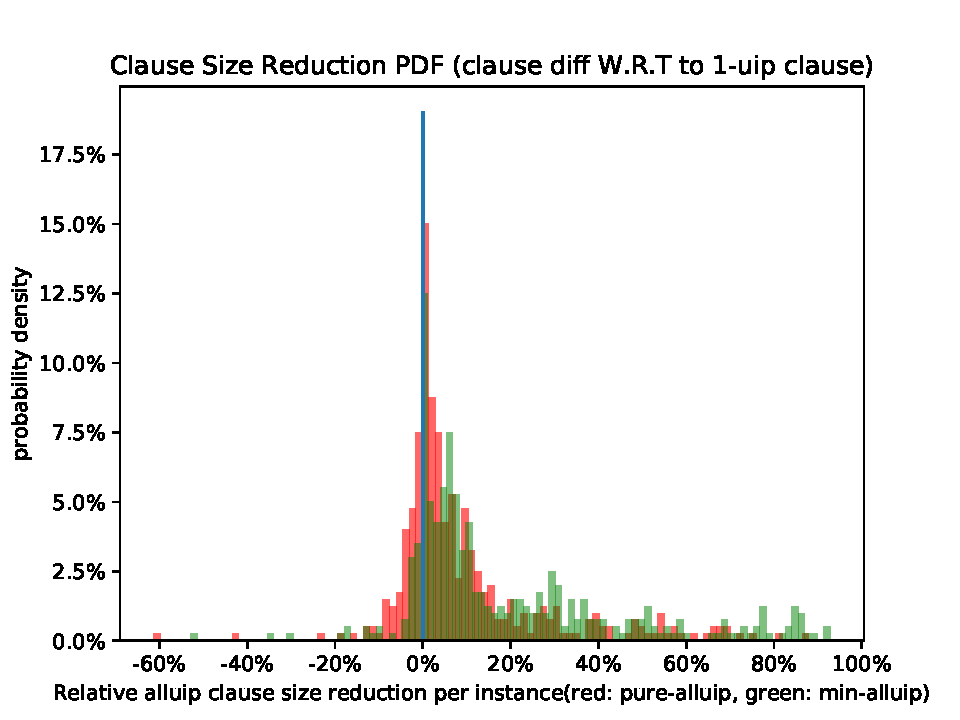
\includegraphics[width=\textwidth]{figures/clause_reduction_PDF.pdf}
   \caption{Relative clause size reduction distribution. The $X$ axis
      indicates the relative size of difference between all-uip and
      1-uip clauses (calculated as
      $\dfrac{|C_1|-|C_i|}{|C_1|}$ ) for
      each instance, and the $Y$ axis shows the probability density.}
       \label{fig:len_pdf}
  \end{minipage}
  & &
  \begin{minipage}[t]{0.5\textwidth}
    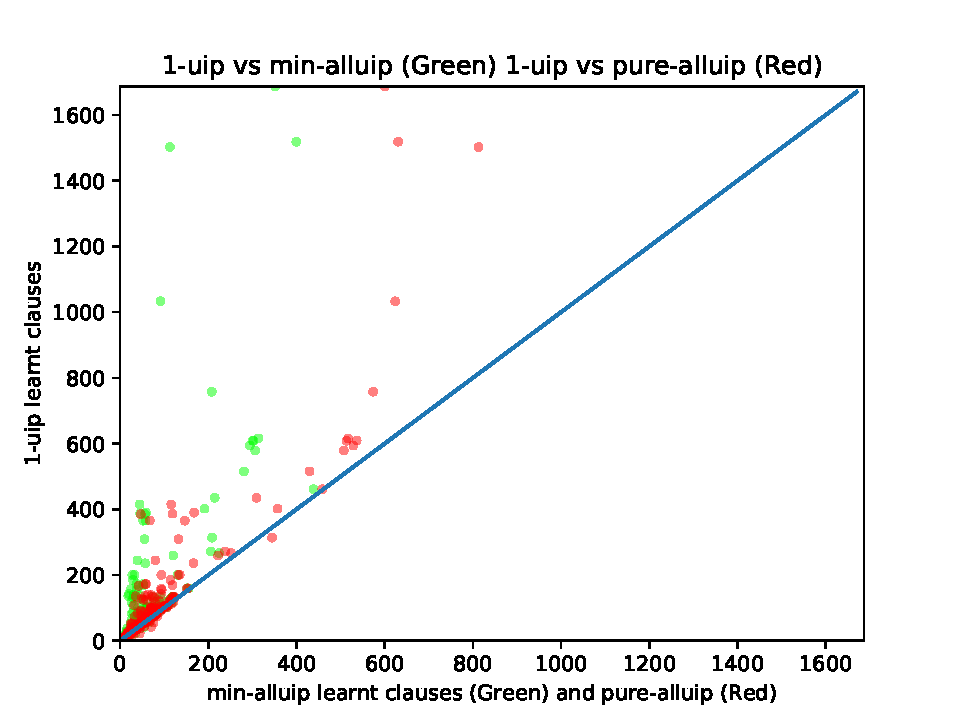
\includegraphics[width=\textwidth]{figures/clause_size_compare.pdf}
    \caption{Average clause size comparison plot. Each point in the
      plot represents an instance. The $X$ and $Y$ axes shows the clause
      length from $\allUip$ and 1-UIP, respectively. Each green (red)
      dot represents an compared instance between $\MapleBase$ and
      $\MapleIUIMin$ ($\allUipPure$).}
      \label{fig:len_compare}
  \end{minipage}

\end{tabular}
}
\end{figure}


%Beside solved instances count and PAR-2 score, we additionally measure
%the average clause size. 
%and clause reduction ratio (both cumulative
%and non-cumulative)\footnote{The cumulative reduction ratio is
%  obtained through learning all clauses with the target learning
%  scheme; Therefore, the reduction is cumulative. The %non-cumulative
%  reduction ratio is obtained by running the target scheme for
%  measurement only (the minimized 1-UIP clause is learned); Therefore,
%  the reduction is not cumulative. }  for each instances. 
%For $\MapleIUIPPure$ and $\MapleIUIMin$, we also captures the $\allUip$
%learning attempted rate and success rate.

%\begin{figure} 
%\begin{center}
%\begin{tabular}{ | m{3.3cm} | m{2cm}| m{2cm} | m{2cm} | m{2.7cm} | } 
%\hline
%Solver & \# solved & PAR-2 & Clause Size & Cl Reduction\% \\ 
%\hline
%$\MapleBase$ & 221 (132, 89) & 5018.89 & 62.6 & 36.53\% \\ 
%\hline
%$\MapleIUIPPure$ & \textbf{228} (135, 93) & \nf{4867.37} & 49.88 & 41.6\%  (42.72\%)\\ 
%\hline
%$\MapleIUIMin$ & 226 (135, 91) & 4890.67 & \textbf{45.2} & \textbf{47.8\% (51.19\%)}\\ 
%\hline
%\end{tabular}
%\end{center}
%\caption{Benchmark results of $\MapleBase$ , $\MapleIUIPPure$  and $\MapleIUIMin$ on SAT2019 %race main track.
%CL Reduction\% is the clause size reduction ratio comparing to non-minimized 1-UIP clauses, %and the values in the brackets are the non-cumulative reduction ratio.}
%\label{fig:t1}
%\end{figure}

%Fig.~\ref{fig:t1} shows that $\allUipPure$ ($\allUipPure$) solved seven
%(five) more instances than the baseline solver with lower PAR-2
%scores. $\allUipPure$ has marginally lower PAR-2 score than
%$\allUipPure$. Both $\allUipPure$ and $\allUipMin$ produce clause with
%significantly smaller size than 1-UIP by 20.4\% and 27.7\%,
%respectively. Fig.~\ref{fig:len_pdf} shows the probability density
%distribution (PDF) of the relative clause size of both i-uip learning
%schemes ($\allUipPure$ in red and $\allUipMin$ in green) for each
%instance. $\allUipPure$ ($\allUipMin$) produces shorter clauses for 77.7\%
%(88.5\%) of instances, and average relative reduction from 1-UIP is
%16.7\% (18.6\%). Fig.~\ref{fig:len_compare} compares the absolute
%clause size of $\allUipMin$, $\allUipPure$ and 1-UIP, and it shows that
%both i-UIP learning schemes in general produce the smaller clauses,
%and the size reduction is more significant for instances with large
%average 1-UIP clause size. Moreover, $\allUipMin$ clauses (indicated in
%5green) is consistently smaller than $\allUipPure$ clauses.

%\nf{ Do we need this?  We additionally looked at the 14 instances
%  solved by $\allUipMin$ but not by 1-UIP. $\allUipMin$ produces smaller
%  clauses for all of them with average relative reduction of 22\% and
%  maximum 77\% (30 vs 135). Seven out of 14 instances has size
%  relative reduction over 30\%. For the 9 instances solved by 1-UIP
%  but not by $\allUipMin$, $\allUipMin$ only produce smaller clause for
%  three instances and with average relative reduction of 3.3\%.}


%\begin{figure} 
%\begin{center} 
%\begin{tabular}{ | m{3.5cm} | m{5cm}| m{3.5cm} | } 
%\hline
%Solver & $\allUip$ attempt rate & $\allUip$ success rate  \\ 
%\hline
%$\MapleIUIPPure$ & 16.1\% & 43.4\% \\ 
%\hline
%$\MapleIUIMin$ & 28.8\% & 59.3\% \\ 
%\hline
%\end{tabular}
%\end{center}
%\caption{Compare $\allUipPure$ and $\allUipMin$ i-uip attempt rate and success rate. %$\allUipMin$ scheme attempted $\allUip$ more frequently, and it is more likely to %successfully produce smaller $C_i$ clause .}
%\label{fig:t2}
%\end{figure}
\subsubsection{Reduced Proof sizes with $\allUip$.}
A learning scheme that yields smaller clauses (lemmas) might also
construct smaller causal proofs. For UNSAT instances, we additionally
compare the size of the optimized DRAT proof from $\allUipPure$,
$\allUipMin$ and 1-UIP schemes. We used the DART-trim tool
\cite{wetzler2014drat} with a 10000 second timeout to check and
optimize every DRAT proof once \footnote{Applying DART-trim multiple
  times can further reduce the proof size until a fix-point. However,
  the full optimization is time consuming and was impractical for our
  experiments.}.

The average optimized DRAT proof from $\allUipMin$ and $\allUipPure$
are 413.2MB and 487.2MB, respectively. Both sizes are significantly
smaller than the average optimized proof size from 1-UIP, 613.9MB.
The average proof size reduction per instance for $\allUipMin$ and
$\allUipPure$ was 17.18\% and 6.9\% compared with 1-UIP, which roughly
correlate with our observed clause size observation in
Fig~\ref{fig:len_pdf}.

%Fig.~\ref{fig:proof_compare} shows the
%absolute proof size comparison between $\allUipMin$ and 1-UIP, and displays a similar trend %as the clause size comparison plot in Fig.~\ref{fig:len_compare}.

%\begin{figure} 
%\begin{center} 
%\begin{tabular}{ | m{3.5cm} | m{5cm}| m{3.5cm} | } 
%\hline
%Solver & optimized proof size (MB) & relative reduction size  \\ 
%\hline
%$\MapleBase$ & 613.9 & 0  \\ 
%\hline
%$\MapleIUIPPure$ & 487.2 & 6.90\% \\ 
%\hline
%$\MapleIUIMin$ & 413.2 & 17.18\% \\ 
%\hline
%\end{tabular}
%\end{center}
%\caption{Optimized UNSAT proof comparison for 1-UIP $\allUipPure$ and $\allUipMin$. %Optimized proof size measures the average absolute proof size in MB, and relative reduction %size measures the average relative reduction for all UNSAT instances.}
%\label{fig:t3}
%\end{figure}

%\begin{figure}
%    \centering
%    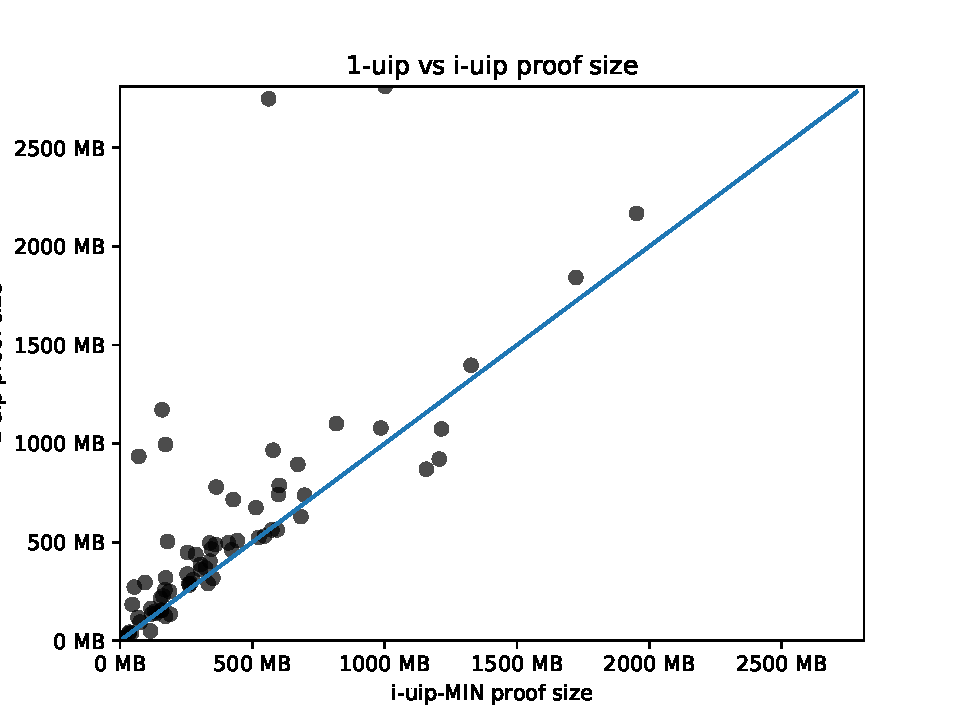
\includegraphics[width=0.8\textwidth]{figures/proof_size_compare.pdf}
%    \caption{Average optimized proof size between 1-uip and $\allUipMin$.}
%    \label{fig:proof_compare}
%\end{figure}

%\subsection{$\allUip$ as a Practical Learning Scheme}
%To evaluate $\allUip$'s effectiveness as a clause learning scheme, we
%re-implement $\allUipMin$ on $\MapleBase$ with the extensions mentioned
%in section~\ref{sec:i-uip}. We evaluated 1-UIP learning and five
%$\allUip$ configurations ( $\allUipMin$, $\allUipPure$, $\allUipAct$,
%$\allUipIn$, and $\allUipEx$) on the SAT Race 2019 main track
%benchmark and reported solved instances, PAR-2 score and average
%clause size.

%Fig.~\ref{fig:t4} summarizes the result of the experiment. Learning
%scheme $\allUipPure$ solved the most overall instances (228) and the
%most UNSAT instances (93). $\allUipAct$ had the lowest PAR-2
%score. $\allUipIn$ solved the most SAT instances (138). $\allUipEx$
%produced the shortest average clause size, but solved the second least
%instances, one more instance than the baseline 1-UIP learning. All
%configurations of $\allUip$ outperformed the baseline 1-UIP scheme in
%solved instances, PAR-2 score and average clause size.


\subsubsection{$\allUip$ on Modern SAT solvers}
To validate $\allUip$ as a practical learning scheme for modern SAT
solvers, we implemented $\allUip$ in the winners of 2017, 2018 and
2019 SAT
Race\cite{luo2017effective,ryvchin2018maple,Stepan2019MapleLCMDistChronoBT}
and in the $\expSAT$\cite{MdSolimul2019expMalpe} ($\expSATShort$)
solver. $\expSATShort$ is a top ten solver from 2019 SAT race which
uses random walk simulation to help branching. We chose $\expSATShort$
because (1) it one of the top solvers in the 2019 SAT Race that does
not use chronological backtracking; and (2) the random walk simulation
branching heuristic is different from local branching heuristic (VSIDS
and LRB) that we have considered in $\allUipAct$, $\allUipIn$, and
$\allUipEx$. We compared these solver's base 1-UIP learning scheme
with $\allUipPure$, $\allUipMin$ and the top two $\allUip$ variants,
$\allUipAct$ and $\allUipIn$, on the SAT Race 2019 main track
benchmark. We report solved instances, PAR-2 score and the average
clause size.

\begin{figure} 
\begin{center}
\begin{tabular}{ | m{3.7cm} | m{4cm}| m{2cm} | m{2.75cm} |  } 
\hline
Solver & \# solved (SAT, UNSAT) & PAR-2 & Avg clause Size \\ 
\hline
SAT 2017 Winner & & & \\
$\MapleSeven$ & 232 (135, 97) & 4755.96 & 61.9  \\ 
\hline
$\MapleSeven$-i-pure & \textbf{244 (146, 98)} +12 & \textbf{4504.18} & 43.76 \\
\hline
$\MapleSeven$-i-min & 240 (144, 96) +8 & 4601.25 & \textbf{36.97} \\ 
\hline
$\MapleSeven$-i-Act & 237 (140, 97) +5 & 4678.434 & 43.62 \\ 
\hline
$\MapleSeven$-i-inclusive & 234 (137, 97) +2 & 4718.03 & 37.96 \\
\hline
\hline
SAT 2018 Winner & & & \\
$\MapleEightShort$ & 236 (138, 98) & 4671.81 & 61.69 \\
\hline
$\MapleEightShort$-i-pure & \textbf{241} (\textbf{142, 99}) +5 & \textbf{4598.18} & 44.19 \\
\hline
$\MapleEightShort$-i-min & 236 (141, 95) +0 & 4683.92 & 38.05 \\ 
\hline
$\MapleEightShort$-i-Act & 240 (141, \textbf{99}) +4 & 4626.99 & 41.16 \\
\hline
$\MapleEightShort$-i-inclusive & 240 (\textbf{142}, 98) +4 & 4602.13 & \textbf{37.52} \\
\hline
\hline
SAT 2019 Winner & & & \\
$\MapleNineShort$ & 238 (140, \textbf{98}) & 4531.24 & 60.91 \\
\hline
$\MapleNineShort$-i-pure & 238 (140, \textbf{98}) +0 & 4519.08 &  43.32\\
\hline
$\MapleNineShort$-i-min & 244 (\textbf{148}, 96) +6 & \textbf{4419.84} & \textbf{36.88} \\
\hline
$\MapleNineShort$-i-Act & 243 (146, 97) + 5 & 4476.73 & 40.65 \\
\hline
$\MapleNineShort$-i-inclusive & \textbf{243} (\textbf{148}, 95) +5 & 4455.76 & 37.02 \\
\hline
\hline
SAT 2019 Competitor & & &\\
$\expSATShort$ & 237 (137, 100)  & 4628.96 & 63.19 \\
\hline
$\expSATShort$-i-pure & 235 (136, 99) -2  & 4668.96 & 48.26 \\
\hline
$\expSATShort$-i-min & 241 (143, 98) +4 & 4524.28 & 46.29 \\ 
\hline
$\expSATShort$-i-Act & 244 (143, \textbf{101}) +7 & \textbf{4460.92} & 47.25 \\
\hline
$\expSATShort$-i-inclusive & \textbf{245} (\textbf{146}, 99) +8 & 4475.76 & \textbf{45.33} \\
\hline
\end{tabular}
\end{center}
\caption{Benchmark results of 1-UIP, $\allUipPure$. $\allUipMin$, $\allUipAct$ and $\allUipIn$ on SAT2019 race main track.}
\label{fig:t5}
\end{figure}

Table~\ref{fig:t5} shows the benchmark result of the $\allUip$
configurations in our suite of modern solvers. Overall, we observed
similar performance gain on all modern solvers as we have seen on
$\MapleBase$ in Fig.~\ref{fig:t4}. More specifically, almost all
configurations improved on solved instance (+4.5 instances in average)
and PAR-2 score (-83.6 in average).  The average clause size reduction
is consistent across all solvers. Each configuration also exhibits
different strength: $\allUipPure$ solved the most instances with the
best PAR-2 score on two solvers, $\allUipMin$ yields small clauses,
$\allUipIn$ solved the most SAT instances, and $\allUipAct$ has stable
performance.


On the SAT 2017 race winner $\MapleSeven$, all four configurations of
$\allUip$ outperformed 1-UIP learning by 12, 8, 5, and 2 instances,
respectively. $\allUipPure$ solved more UNSAT and SAT instances while
the other configurations improved on solving SAT instances. The clause
size reduction of $\allUip$ is more significant on $\MapleSeven$
than on to $\MapleBase$.
%This may suggests that $\allUip$ and the recent
%learnt clause minimization approach~\cite{} synergies well because
%i-UIP clauses are shorter with more common literals which allows
%vivification~\cite{} to prune literals more aggressively through unit
%propagation.

The SAT 2018 race winner$\MapleEightShort$ uses chronological
backtracking (CB) for long distance backtracks. Three out of four
$\allUip$ configurations outperformed 1-UIP by 5, 4 an 4 instances,
respectively.
%$\MapleEightShort$ improved from $\MapleSeven$ by using
%chronological backtracking (CB) for long distance
%backtracks. Therefore, we used $\allUip$-CB extension for all $\allUip$
%configurations. 

%The results indicates that the improvement of $\allUip$
%is slightly shadowed by the adoption of CB. More specifically, we
%believe CB prevents decision levels from being compressed through the
%process of backtracking and literal assertion. The shorter i-UIP
%clauses can bring related literals closer, which in turns compresses
%the assertion stack and the decision levels. However, since CB
%discourages long distance backtracking, the effect of learning shorter
%clauses is shadowed until a full restart.  We believe we have observed
%an interesting interaction effect that shows the limitations of both
%CB and $\allUip$ learning for future research.

On the SAT 2019 race winner $\MapleNineShort$, three out of four
$\allUip$ configurations solved instances 6, 5 and 5 more instances
than 1-UIP, respectively. $\MapleNineShort$ prioritizes clauses that
are learned multiple times. We observed that clauses learnt from
$\allUip$ configurations are less likely to be duplicated. As an
example, $\allUipMin$ in average, added 12\% less duplicated clauses
into the core clause database than 1-UIP. This observation is
surprising, and the cause is unclear.

%One possible explanation is that
%$\allUip$ learning can reduce an 1-UIP clause to different i-UIP clauses
%for different assertion trails. Therefore, the solver is less likely
%to learn the same i-UIP clauses.

On $\expSATShort$, three out of four $\allUip$ configurations solved
4, 7 and 8 more instances than 1-UIP learning. We noticed that
$\allUipAct$ and $\allUipIn$ show significant better performance than
$\allUipMin$ and $\allUipPure$ on this solver. The random walk
simulation branching heuristic, however, didn't impact the performance
of $\allUip$ schemes significantly.
%$\allUip$ to solve the similar amount of instances with close PAR-2
%scores because the additional random walk exploration allows the
%learning schemes to partially sidestep the activity problem; hence,
%the learning adjustment for variable activities should have less
%impact on the solver's performance. However, we instead, observed that
%both $\allUipAct$ and $\allUipIn$ outperformed the default i-UIP
%learning scheme. One possible explanation is that $\allUipAct$ and
%$\allUipIn$ schemes could easily overcompensate variable activities
%for i-UIP clauses, and $\expSATShort$'s random walk exploration could
%use future search information to mitigate the negative effects of our
%overcompensation.

\bibliography{sat}{}
\bibliographystyle{splncs04}
\end{document}

